\documentclass[tikz,border=4pt]{standalone}
\usepackage[T1]{fontenc}
\usepackage{lmodern}
\usetikzlibrary{positioning,arrows.meta,fit,backgrounds,calc}
% Plain-language companion to fig-register.tex, for popular outputs (blog, talk, post).
% Same structure and colours; every hedge of the paper figure kept, in plain words.
\definecolor{ver}{HTML}{1F7A7A}
\definecolor{verbg}{HTML}{E6F2F2}
\definecolor{val}{HTML}{B5651D}
\definecolor{valbg}{HTML}{FBEEDD}
\definecolor{struct}{HTML}{555555}
\begin{document}
\sffamily\footnotesize
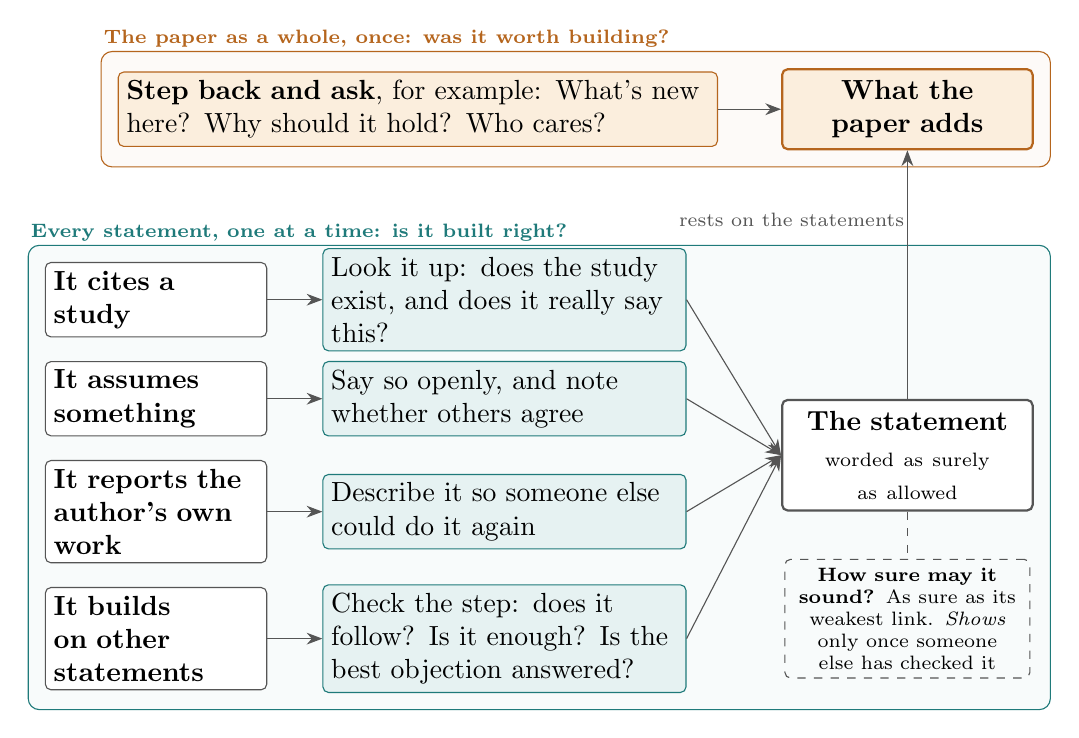
\begin{tikzpicture}[
  node distance=3mm and 7mm,
  every node/.append style={execute at begin node={\hyphenpenalty=10000 \exhyphenpenalty=10000 }},
  ground/.style={draw=struct, rounded corners=2pt, text width=2.6cm, minimum height=9mm, align=left, inner sep=3pt, fill=white},
  check/.style={draw=ver, rounded corners=2pt, text width=4.4cm, minimum height=9mm, align=left, inner sep=3pt, fill=verbg},
  claim/.style={draw=struct, thick, rounded corners=2pt, text width=2.9cm, align=center, inner sep=4pt, fill=white},
  arr/.style={-{Stealth[length=2mm]}, struct},
  band/.style={font=\scriptsize\bfseries, anchor=south west, inner sep=1pt},
]
% --- Each statement, one at a time ---
\node[ground] (src) {\textbf{It cites a study}};
\node[ground, below=of src] (decl) {\textbf{It assumes something}};
\node[ground, below=of decl] (own) {\textbf{It reports the author's own work}};
\node[ground, below=of own] (oth) {\textbf{It builds on other statements}};

\node[check, right=of src] (csrc) {Look it up: does the study exist, and does it really say this?};
\node[check, right=of decl] (cdecl) {Say so openly, and note whether others agree};
\node[check, right=of own] (cown) {Describe it so someone else could do it again};
\node[check, right=of oth] (coth) {Check the step: does it follow? Is it enough? Is the best objection answered?};

\foreach \g/\c in {src/csrc, decl/cdecl, own/cown, oth/coth} \draw[arr] (\g) -- (\c);

\node[claim, right=12mm of $(cdecl.east)!0.5!(cown.east)$] (claim) {\textbf{The statement}\\[1pt] \scriptsize worded as surely as allowed};
\foreach \c in {csrc, cdecl, cown, coth} \draw[arr] (\c.east) -- (claim.west);

\node[draw=struct, dashed, rounded corners=2pt, text width=2.9cm, align=center, inner sep=3pt, below=6mm of claim, font=\scriptsize] (tier)
  {\textbf{How sure may it sound?} As sure as its weakest link. \emph{Shows} only once someone else has checked it};
\draw[struct, dashed] (claim) -- (tier);

\begin{scope}[on background layer]
  \node[fit=(src)(oth)(coth)(claim)(tier), draw=ver, rounded corners=4pt, inner sep=6pt, fill=ver!3] (verband) {};
\end{scope}
\node[band, text=ver] at (verband.north west) {Every statement, one at a time: is it built right?};

% --- The paper as a whole, once ---
\node[claim, fill=valbg, draw=val, anchor=south] (contr) at ($(verband.north -| claim)+(0,12mm)$) {\textbf{What the paper adds}};
\node[draw=val, rounded corners=2pt, text width=7.4cm, align=left, inner sep=3pt, fill=valbg, left=8mm of contr] (whet)
  {\textbf{Step back and ask}, for example: What's new here? Why should it hold? Who cares?};
\draw[arr] (whet) -- (contr);
\draw[arr] (claim.north) -- node[pos=0.72, left, font=\scriptsize, text=struct, fill=white, inner sep=1pt] {rests on the statements} (contr.south);

\begin{scope}[on background layer]
  \node[fit=(whet)(contr), draw=val, rounded corners=4pt, inner sep=6pt, fill=val!3] (valband) {};
\end{scope}
\node[band, text=val] at (valband.north west) {The paper as a whole, once: was it worth building?};
\end{tikzpicture}
\end{document}
